

\documentclass[a4paper, 11pt, english, fleqn]{article}
\usepackage[utf8]{inputenc}
\usepackage{babel}
%\usepackage{ngerman}
\usepackage{coordsys,logsys,color}
\usepackage{fancyhdr}
\usepackage{hyperref}
\usepackage{texdraw}				
\usepackage[T1]{fontenc}					
\usepackage{amsmath,amsfonts,amssymb}	
\usepackage[normalem]{ulem}	
\usepackage{listings}
\usepackage{graphicx}
\usepackage{enumitem}
\usepackage[paper=a4paper,left=35mm,right=35mm,top=35mm,bottom=30mm]{geometry}

\hypersetup{colorlinks=true, breaklinks=true, linkcolor=darkblue, menucolor=black, urlcolor=darkblue, citecolor=darkblue}

\pagestyle{fancy}

\renewcommand{\familydefault}{cmss}

\definecolor{fgcgray}{rgb}{0.4, 0.4, 0.4}
\definecolor{darkblue}{rgb}{0,0, 0.4}
\newcommand{\titlefont}[1]{\textcolor{black}{\fontseries{bx}\fontshape{n}\fontsize{30}{0pt} \selectfont #1}}
\newcommand{\titlepagef}[1]{\textcolor{black}{\fontseries{bx}\fontshape{n}\fontsize{14}{0pt} \selectfont #1}}

\newcommand{\gloss}[1]{\textcolor{glossb}{\fontsize{11}{0pt}\selectfont #1}}

\newlist{aims}{enumerate}{1}
\setlist[aims,1]{
	label={Aim~\arabic*},
	leftmargin=*,
	align=left,
	%labelsep=1mm,
	font=\bfseries
}

\addtolength{\oddsidemargin}{-1.0cm}
\addtolength{\evensidemargin}{-1.0cm}
\addtolength{\headwidth}{2.0cm}
\addtolength{\textwidth}{2.0cm}

\setlength{\parindent}{0cm}

\renewcommand{\labelitemi}{$\circ$}
\renewcommand{\labelitemii}{$\diamond$}

\newcommand{\spaceline}[1][8pt]{\vskip #1}
\newcommand{\attrname}[1]{\textcolor{fgcgray}{\scriptsize #1}}

\newcommand{\comment}[1]{\spaceline[5pt] \textcolor{fgcgray}{\scriptsize #1} \spaceline[15pt]}

\makeatletter

\newcommand*{\project}[1]{\gdef\@project{#1}}


\def\@maketitle{
  %\begin{titlepage}
   
  \begin{center}
      \titlepagef{Software-Project 2017}
      \spaceline
  \end{center}
  
  \begin{center}
      \parbox{\textwidth}{
        \spaceline
        \centering{\titlefont{Detailed Design}}
        \par
        \spaceline
      }
  \end{center}
  
  \begin{center}
  	\titlepagef{Real-Time Mesh Utilities}
  	\spaceline[2em]
  \end{center}
  
  \begin{center}
  \begin{tabbing}
  Petros Simidyan \qquad \=
  Blerta Hamzallari \qquad \=
  Felix Griesau \qquad \=
  Marco Klamke \\
  Julius Lerm
  \>Lars Debor
  \>Simon Heinke  
  \>Sugandha Sachdeva
  \end{tabbing}
  \end{center}
 
  
  \spaceline[3em] {
    \begin{flushright}
    \begin{tabular}[t]{rl}
      \attrname{last change:} & \@date
    \end{tabular}
    \end{flushright}
    \par
  }
  \spaceline[5.5em]
  %\end{titlepage}
}

\begin{document}

\pagenumbering{gobble}
	
\lhead{\sc{Detailed Design: RTMU}}	
\title{Detailed Design: RTMU}
\vspace{3 in}
\maketitle


\includegraphics[width = \linewidth]{figures/mne-cpp.png}

\clearpage

\pagenumbering{arabic}

\tableofcontents

\clearpage
\section{General Architecture}
The features of the mesh utilities are divided into two classes...

\clearpage

\section{GeometryInfo}

The class \textit{GeometryInfo} holds all needed functions for the Surface Constrained Distance Calculation (from now on abbreviated with SCDC) and the Sensor Projecting (see Functional Specification for further details). Since all functions are static, the class itself does not have to be instantiated, thus the class also is declared static and the default constructor is forbidden. The class \textit{GeometryInfo} does not have any class members.

\begin{figure}[h]
	\begin{center}
		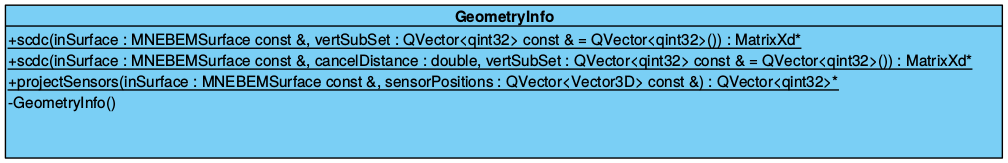
\includegraphics[width=16cm]{figures/geometryinfoclassdiagram.png}
		\caption{Interface of GeometryInfo}
	\end{center}
\end{figure}

\subsection{Member Functions}

\subsubsection{scdc}
The method \textit{scdc} originally was thought to receive only one input argument, i.e. the MNEBemSurface (object that holds the needed adjacency information). Based on this, it was supposed to calculate the full distance table. Since the latter would have needed around 160 gigabyte of memory for some meshes, it was decided that the method also receives a subset of vertices. It then only calculates all distances for each vertex of said subset. The subset argument is defaulted with an empty vector, in case a subset could not be provided or is not wanted.\\
After first tests revealed that an unrestricted distance calculation would take far too long, a third argument was introduced: A double value that acts as a distance threshold and thus restricts the distance calculation to vertices which lie within the said radius. This seems a bit imprecise or careless at first glance, but it actually is reasonable for this specific application: Bilateral stimulation of cells inside the brain only occurs up to a certain distance. The third argument is defaulted with the maximum double-value, in case a distance threshold could not be provided or is not wanted.\\
After these restrictions and adaptions were agreed upon, the question which algorithm to choose arose.
While P.a.R's algorithm had the best asymptotic run-time, further research revealed that an implementation would go far beyond the scope of this project, since the algorithm uses several other algorithms as subroutines (such as Jarnik and Prim). Another possible candidate for solving the problem was Thorups algorithm. Testing of a publicly available implementation showed that it actually did worse than another algorithm, when the above mentioned restrictions to the problem were applied. The one algorithm that resulted in a lower computation time was an iterative version of Dijkstras algorithm (see below for more details).\\
Since two instances of iterative Dijkstra would not interfere with each other (because they work on different columns of the distance table), it was decided for the \textit{scdc} method to start several threads. Before any threads are started, the distance table is allocated. According to the number of available threads (or cores, depending on hyperthreading etc.), the passed subset of vertices gets split into equally sized subvectors, whose limiting indices are then passed to an instance of iterative Dijkstra. 

\subsubsection{iterativeDijkstra}
The method \textit{iterativeDijkstra} receives six input arguments: Firstly a pointer to the distance table which the results are to be written to. Secondly, a reference to an MNEBemSurface which holds the necessary adjacency information. As described above, the \textit{iterativeDijkstra} method receives a vector of indices which point to vertices inside the MNEBemSurface. Added to that, it gets passed two indices which limit the section of said vector that the respective instance of \textit{iterativeDijkstra} is responsible for.
Since the external requirements (i.e. low computation time and overall high efficiency) induce some restrictions (see description of \textit{scdc} for more details), a distance threshold gets passed as the sixth argument. Because Dijkstras algorithm is so well known, its general implementation is not described in this document. Apart from a standard version of Dijkstras algorithm, \textit{iterativeDijkstra} ignores vertices that have a higher distance than said threshold, that means it does not check their neighbors for possibly better paths.\\
This method is private, since begründung

\subsubsection{projectSensors}
asdf

\subsubsection{nearestNeighbor}
asödlkfj

\subsubsection{matrixDump}
This method is implemented for testing and verifying purposes only. It receives a MatrixXd and a string. It then writes the content of the matrix into a file that is named with said string.

\subsubsection{squared}
This method is implemented for better readability only, thus it is declared private. It receives a double-value and returns it squared. In order to avoid efficiency losses through stack frames, it is declared inline.

\clearpage


\section{Interpolation}
The class \textit{Interpolation} holds all ...

\begin{figure}[h]
	\begin{center}
		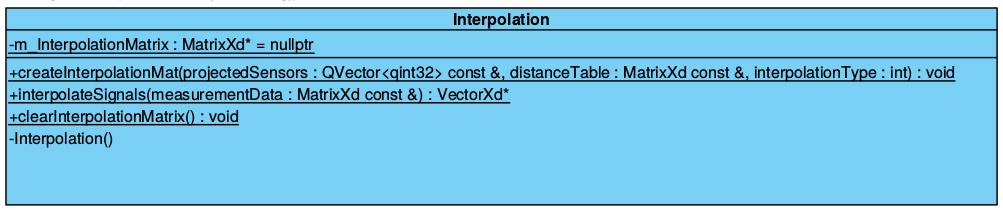
\includegraphics[width=16cm]{figures/interpolationclassdiagram.png}
		\caption{Interface of Interpolation}
	\end{center}
\end{figure}

\subsection{Member Objects}

\subsubsection{Weight Matrix}

\subsection{Member Functions}

\subsubsection{createInterpolationMatrix}
asdf

\subsubsection{interpolateSignal}
The method \textit{interpolateSignal} calculates the full

\subsubsection{clearInterpolationMatrix}
The method \textit{clearInterpolationMatrix} resets the weight matrix, i.e. frees all memory allocated for the respective member object.

\subsubsection{getResult}
This method is implemented in case the calculated weight matrix is needed as an object itself. It returns a smart pointer to the weight matrix (see member objects for more details).

\subsubsection{linear, gaussian, square}
These methods are implemented to provide a minimal preset of functions to use during the calculation of the interpolation weight matrix (see method \textit{createInterpolationMatrix} for more details).

\clearpage

\section{Glossary}
mesh
MatrixXd
dijkstra verweis,
jarnik und prim
  
\end{document}
